
\chapter{Allgemeine Untis Bedienungshinweise}

Guten Tag! Ich habe ein kleines Handbuch erstellt die hoffentlich der Einstieg oder Umstieg in Untis 2015 erleichtert.\\
\\
Untis 2015 bietet viele neue Funktionen. Sie erleichtern die Arbeit mit Untis und bieten viele Einstellungsmöglichkeiten um die Darstellung bequemer und persönlicher zu gestalten. In diesem Kapitel hoffe ich euch behilflich zu sein, um Untis ihre persönliche Bedürfnisse anzupassen und der Umgang mit der Vielfalt an Ansichten zu erleichtern.\\
\\

\section{Ribbon Oberfläche und neue Menüführung}

Das erste was man auffällt bei Untis 2015 ist der Umstieg auf der, für den meisten, vertraute Ribbon-Oberfläche, die bei Microsoft Produkte üblich ist.

\begin{figure}[h]
	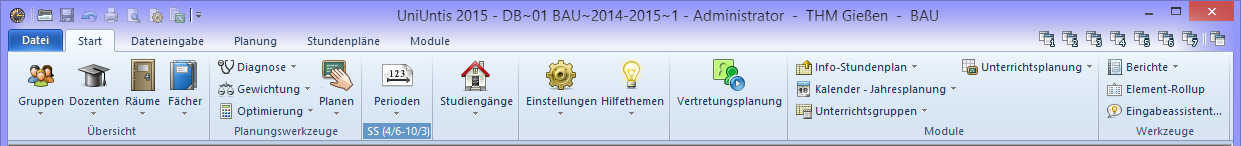
\includegraphics[width=1\textwidth]{ribbon-menu}
	\vspace{-15pt}
	\caption{Ribbon Oberfläche}
	\label{fig:ribbon}
\end{figure}

\noindent
Was man auch auffällt es gibt des wegen weniger Hauptmenüpunkte und viele der Untermenüpunkte werden sofort sichtbar welches die Navigation deutlich erleichtert. Auch viele der Ressourcen-bezogene Menüpunkte wurden unter die entsprechende Ressourcen konsolidiert. Beispielsweise sind die Ansichten für Gruppenverwaltung, Unterrichte (Gruppen-bezogen), und sämtlicher Gruppenpläne jetzt Untermenüpunkte von Gruppen.

\subsection{Menü Personalisierung}

Eine weitere Neuigkeit ist die Fähigkeit die Menüleiste anzupassen, unter Anderem die in der Schnellzugriff-Leiste angebotenen Ansichten, die deren Positionierung, und die Anzeige der Ribbon-Oberfläche.\\

\begin{wrapfigure}{r}{0.4\textwidth}
	\vspace{-4pt}
	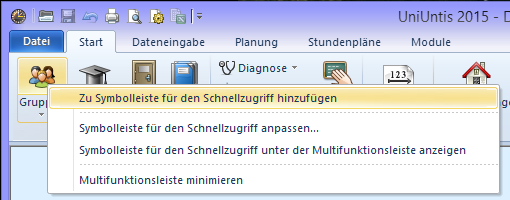
\includegraphics[width=.38\textwidth]{context-menu}
	\vspace{-5pt}
	\caption{Kontext Menü}
	\label{fig:context-menu}
	\vspace{50pt}
	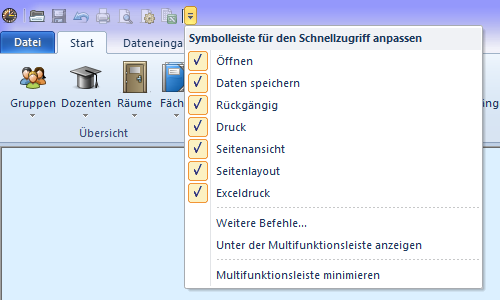
\includegraphics[width=.38\textwidth]{remove-quick-access-item}
	\vspace{-5pt}
	\caption{Vordefinierte Symbole\newline Entfernen}
	\label{fig:remove-quick-access-item}
	\vspace{4pt}
\end{wrapfigure}

\noindent
Um Ansichten der Schnellzugriff-Leiste hinzuzufügen öffnet man den Kontext Menü (Rechtsklick) und klickt auf den ersten Eintrag 'Zu Symbolleiste für den Schnellzugriff hinzufügen'. Hiermit kann man häufig verwendete Ansichten schneller, bzw. ohne die Menüführung zu verwenden, öffnen.\\
\\
Es gibt zwei Methoden Elemente aus der Schnellzugriff-Leiste zu entfernen. Wenn Sie das Symbol nicht standardmäßig angeboten wird, i.e. Sie haben das Symbol selbst hinzugefügt, soll man auch über das Kontext Menü entfernen. Wenn man Rechtsklick auf einem solchen Symbol macht kommt als erstes Option 'Aus Symbolleiste für den Schnellzugriff entfernen', das Klicken dieser Option entfernt das Symbol von der Leiste.\\
\\
Um vordefinierte Symbole wie 'Öffnen' oder 'Datei Speichern' zu entfernen klickt man auf das kleine Pfeil nach unten Symbol direkt rechts von der Leiste. Diese öffnet eine neue Kontext Menü in dem die bereits erhaltene Symbole dargestellt werden mit einem Häkchen davor. Um die unerwünschte Symbole aus der Liste zu entfernen sollen nun die entsprechende Häkchen entfernt werden.\\
\\
Da die Ribbon-Oberfläche von der Fläche der Arbeitsfläche weg nimmt, hat Gruber und Petters auch über den Kontext Menü die Möglichkeit angeboten diese zu minimieren. Dies hat als Folge, dass die Ribbon-Oberfläche nur sichtbar wird wenn man einer der Hauptmenüpunkte anklickt. Das Standardverhalten kann man von überall in der Menüleiste durch das entfernen der entsprechende Häkchen vom Kontext Menü wiederherstellen.\\
\\
Letztlich kann man auch die Schnellzugriff-Leiste unterhalb der Ribbon-Oberfläche darstellen lassen, in dem man im Kontext Menü der dritte Punkt 'Symbolleiste für den Schnellzugriff unter der Multifunktionsleiste anzeigen' klickt. So eingestellt kann man die Leiste auf ihre Ursprungsposition bringen in dem man nochmal auf den dritten Punkt der Kontext Menü klickt.\\
\\
Weiter fortgeschrittene Personalisierungseinstellungen befinden sich im Schaltfläche Personalisierung, Sektion \ref{sec:advanced-quick-access}.

\subsection{Standard Fenstergruppen}

\begin{wrapfigure}{r}{0.4\textwidth}
	\vspace{-14pt}
	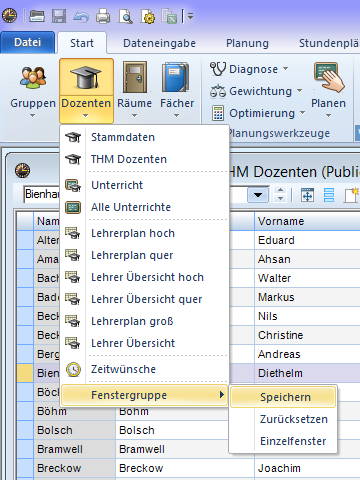
\includegraphics[width=.38\textwidth]{default-window-grouping}
	\vspace{-5pt}
	\caption{Felder der Ansicht Icon}
	\label{fig:default-window-grouping}
	\vspace{-10pt}
\end{wrapfigure}

Eine weitere Neuigkeit gebunden mit der Konsolidierung der Ressourcen-Ansichten sind die Standard Fenstergruppen. Wenn man auf die große Symbolen der Hauptressourcen klickt kommen erstmal eine vordefinierte Gruppierung von Ansichten, die mit dieser Ressource zu tun haben, hoch. Zum Beispiel, durch ein Klick auf das Tür Symbol werden alle bereits geöffnete Ansichten geschlossen und die Ansichten Stammdaten, Zeitwünsche, Raumplan Hoch, und Unterricht geöffnet.\\
\\
Obwohl die voreingestellte Ansichten nicht zu gebrauchen sind, deuten sie an welche Fülle man in die Arbeitsfläche packen kann und können sehr leicht an Ihre persönliche Bedürfnisse angepasst werden. Um eine solche Fenstergruppe zu erstellen, öffnen Sie vorerst die Ansichten und Formaten mit den Sie gerne arbeiten würden und verteilen sie auf der Arbeitsfläche wie sie Ihnen am besten gefallen.\\

\section{Fensterbedienung}

\begin{wrapfigure}{r}{0.4\textwidth}
	\vspace{-14pt}
	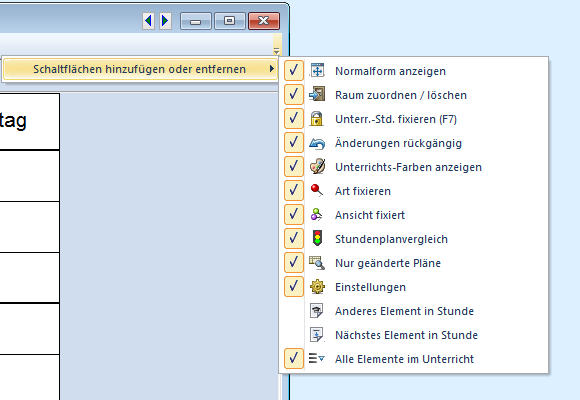
\includegraphics[width=.38\textwidth]{window-personalization}
	\vspace{-5pt}
	\caption{Fenster Personalisierung}
	\label{fig:window-personalization}
\end{wrapfigure}

Ab Untis 2015 sind die Symbolleisten der Fenstern nicht mehr frei verschiebbar, dafür kann man ähnlich wie die Schnellzugriff Leiste ein und ausblenden über der Pfeil nach unten an der rechte Seite der jeweilige Symbolleiste. Ein klick darauf öffnet ein Menü, dessen Länge von der Anzahl der nicht angezeigte Symbolen abhängig ist. Wichtig ist hier der letzter Eintrag, 'Schaltflächen hinzufügen oder entfernen'.\\
\\
Dieser blendet eine weitere Menü ein mit dem man die angezeigt Elemente das eigene Vorlieben anpassen kann. Wobei hier die Elemente, die zur Auswahl stehen, vom jeweiligen Fenstertyp abhängig sind. Stammdaten Fenster werden beispielsweise teilweise andere Bedienungssymbole zur Verfügung haben als Übersichtspläne. Es ist sogar so, dass zwischen unterschiedlichen Fenstertypen unterschiedliche Funktionalität hinter die gleiche Symbolik steckt. Mehr Informationen dazu später in diesem Sektion und die ansichtsspezifischen Sektionen.\\
\\
Im ersten Teil der Sektion werde ich die mit der überarbeitete Auswahlbox kurz erläutern. Danach werden die Symbolleiste verbundene Aktionen angesprochen. Diese handelt sich um Aktionen die über diese Leiste abgeschlossene Aktionen durchführen oder weitere Schnittstellen öffnen. Ich nenne diese Symbolleiste Aktionen. Im dritten Teil werde ich Bedienungsfunktionen, die erst mit der Eingabe und Anzeige der Daten einleuchten können, beschreiben. Ich nenne solche Funktionen Fenster-Aktionen.

\subsection{Auswahl und Suche}

Die Auswahlbox in Untis Version 2015 wurde deutlich überarbeitet und bietet viele neue Verbesserungen. Erstens die statische Auswahl wächst nun dynamisch in die Breite. Damit werden die, für gewöhnlich aussagekräftigere, Langnamen immer angezeigt.\\


\begin{wrapfigure}{r}{.4\textwidth}
	\vspace{-13pt}
	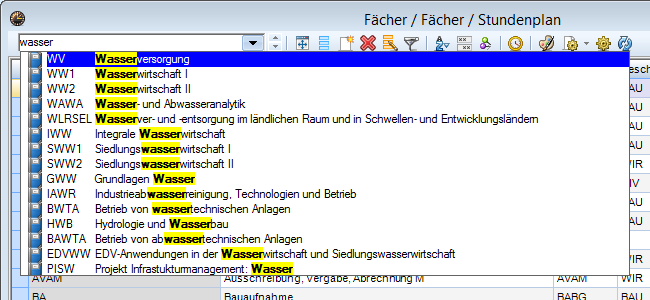
\includegraphics[width=.38\textwidth]{search-field}
	\vspace{-5pt}
	\caption{Suchen}
	\label{fig:search-field}
\end{wrapfigure}

\noindent
Die Auswahlbox, als solches, ist jedoch nebensächlich geworden, denn beim Eintippen werden die kompletten Inhalte der Kurz- und Langnamen durchgesucht. Bei der Eingabe eines einzelnen Zeichen fängt Untis schon an die Ergebnisse einzugrenzen und diese werden auch sofort in der Drop-Down Liste angezeigt. Sprich bei vielen Ressourcen ist es immer schneller die Auswahlbox als Suchfeld zu benutzen.

\subsection{Symbolleiste Aktionen}

Hier werden die typischen Symbole der Stammdaten-, Unterrichts- und Stundenplansansichten kurz erläutert. Symbole die für uns überflüssig sind werden nicht angesprochen.\\

\subsubsection{Alle Elemente im Unterricht}
{\small\textit{verfügbar in Einzelplan Ansichten\\}\par}

\begin{wrapfigure}{r}{.06\textwidth}
	\vspace{-50pt}
	
\includegraphics[width=.06\textwidth]{alle-elemente-im-unterricht-symbol}
	\vspace{-35pt}
\end{wrapfigure}

\noindent
Dieser erzeugt einen kleinen Reiterleiste im oberen linken Ecke eines Einzelplans. Sollte man einer Unterrichtsstunde im Plan auswählen werden Reiter erstellt und dieser Reiterleiste hinzugefügt. Man kann auf die Elemente dieser Leiste klicken um die Einzelpläne der verbundene Ressourcen schnell anzuschauen. Standardmäßig eingeschaltet, das ausschalten lässt der Reiter verschwinden und, sollte man einen anderen Plan angeschaut haben, man wird zum Ursprungsplan zurückgebracht.\\

\subsubsection{Änderungen Rückgängig}
{\small\textit{explizit verfügbar in allen Stundenplan Ansichten\\}\par}

\begin{wrapfigure}{r}{.05\textwidth}
	\vspace{-50pt}
	
\includegraphics[width=.05\textwidth]{anderungen-ruckgangig-symbol}
	\vspace{-35pt}
\end{wrapfigure}

\noindent
Änderungen in Untis werden Protokolliert und können rückgängig gemacht werden. Stundenpläne haben diesen Symbol in der Symbolleiste stehen. Das Rückgängig-Machen kann aber in jede Ansicht verwendet werden. In der Ansichten in dem das Symbol nicht steht kann man entweder STRG + Z drücken oder in das Symbol in der Schnellzugriff Leiste betätigen.\\
\\
\textbf{Vorsicht}: \textit{Diese Funktion protokolliert im aktuellen Stand den zugewiesenen Räume in der Planung nicht mit! Manuell zugewiesene Räume gehen verloren!}

\subsubsection{Ansicht Fixiert}
{\small\textit{verfügbar in allen Fenster Ansichten\\}\par}

\begin{wrapfigure}{r}{.05\textwidth}
	\vspace{-50pt}
	
\includegraphics[width=.05\textwidth]{ansicht-fixiert-symbol}
	\vspace{-35pt}
\end{wrapfigure}

\noindent
Diese Aktion beeinflusst das Verhalten des Fensters in Abhängigkeit von der ausgewählten Elemente andere Fenster. Standardmäßig ist dieser ausgestellt, sprich das Fenster wird von Benutzerinteraktion mit anderen Fenstern beeinflusst. Dies kann oft von Vorteil sein, z.B. wenn man Ressourcenpläne von unterschiedlichen Typen gleichzeitig untersucht. Sobald man die Pläne zweier Ressourcen des gleiche Ressourcentyps untersucht ist es ratsam einer diesen zu fixieren, sonst passen sich die ausgewählte Ressourcen der Pläne an.\\

\subsubsection{Einstellungen}
{\small\textit{verfügbar in allen Fenster Ansichten\\}\par}

\begin{wrapfigure}{r}{.05\textwidth}
	\vspace{-50pt}
	
\includegraphics[width=.05\textwidth]{einstellungen-symbol}
	\vspace{-35pt}
\end{wrapfigure}

\noindent
Obwohl verfügbar in allen Fenster Ansichten, wegen der unterschiedlichen Natur dieser, haben alle Einstellungen Symbolen anderer verbundene Funktionalität.\\
\\
Bei Stammdaten und Unterricht Ansichten sind die Einstellungen hauptsächlich mit der Auswahl der Schriftart, -größe und - stil zu tun. Bei Unterricht Ansichten kann man zusätzlich entscheiden ob die Summenezeile und geerbte Kennzeichen angezeigt werden sollten. Die option ``nur eine Woche" scheint die Anzeige der Unterrichtstunden einzugrenzen auf die Stunden die in der erste Schulwoche stattfinden, ich habe keine Möglichkeit gesehen weitere Wochen anzusehen und bitte diese Option nicht zu setzten.\\
\\
Bei Stundenplan Ansichten öffnen sich weitere Einstellungen die ich später im Sektion !!!!!!! näher erklären werde.\\

\subsubsection{Erweitertes Entkoppeln}
{\small\textit{verfügbar in Unterricht Ansichten\\}\par}

\begin{wrapfigure}{r}{.05\textwidth}
	\vspace{-50pt}
	
\includegraphics[width=.05\textwidth]{erweitertes-entkoppeln-symbol}
	\vspace{-35pt}
\end{wrapfigure}

\noindent
Dieser Symbol öffnet ein das Entkoppeln Ansicht, wo man ausgewählte Unterrichtskopplungszeilen zu eigenständige Unterrichten umgestalten kann. Mehr dazu im Sektion !!!!!!!.\\

\subsubsection{Farbe des Elements}
{\small\textit{verfügbar in Stammdaten und Unterricht Ansichten\\}\par}

\begin{wrapfigure}{r}{.05\textwidth}
	\vspace{-50pt}
	
\includegraphics[width=.05\textwidth]{farbe-des-elements-symbol}
	\vspace{-35pt}
\end{wrapfigure}

\noindent
Öffnet die Farbe Ansicht. Hier kann man Elemente Vorgrund (Schrift) sowie Hintergrund Farben zuweisen. Untis hat von sich aus eine Palette mit 48 Farben und lässt bis zu 12 eigene definieren. Man kann die Farbe-Einstellungen eines Elements leicht entfernen in dem man ein Häkchen bei keine Farben setzt. Sofern man den Ansicht noch nicht geschlossen hat kann man die bisherige Einstellungen durch das entfernen des Häkchens wiederherstellen. Desweiteren kann man Stammdaten Elemente so einstellen, dass neue automatisch Farben zugewiesen bekommen.\\

\subsubsection{Felder der Ansicht}
{\small\textit{verfügbar in Stammdaten und Unterricht Ansichten\\}\par}

\begin{wrapfigure}{r}{.05\textwidth}
	\vspace{-50pt}
	
\includegraphics[width=.05\textwidth]{felder-der-ansicht-symbol}
	\vspace{-35pt}
\end{wrapfigure}

\noindent
Untis, von sich aus, verlangt nur das nötigste an Daten, um diese Anzulegen, bei Stammdaten nur der Name (Kurzname) der Ressource und bei Unterrichte nur eine Anzahl der zu haltende Stunden. Jedoch hat jede Ressourcentyp ein Standardsatz an Zusatzfelder die per Default eingeblendet sind. Diese sind für unsere Zwecke aber nicht ausreichend und ansatzweise auch nicht passend.

\begin{wrapfigure}{r}{0.4\textwidth}
	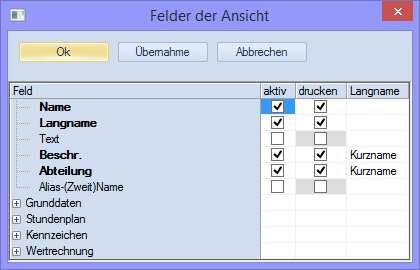
\includegraphics[width=.38\textwidth,right]{felder-der-ansicht}
	\vspace{-15pt}
	\caption{Felder der Ansicht}
	\label{fig:felder-der-ansicht}
\end{wrapfigure}

\noindent
Damit wir möglichst aussagekräftige Daten haben im System, müssen die Felder erst angepasst werden. Diese werden über das Symbol, bzw. der Ansicht ``Felder der Ansicht" eingeblendet. Hier kann man überflüßige Angaben, wie Hohlstunden, ausblendet und wichtige wie Schulübergreifender Name eingeblendet werden. Die spezifische Felder werden bei der jeweilige Ansicht näher erläutert.\\
\\
Sofern die Angabe eine weitere verwaltete Ressource ist kann man auch auswählen wie die Angabe dieser Ressource erfolgen soll. Möglich sind der ``Kurzname", der ``Langname" (bzw. ``Nachname") oder beide Namen mit einem Schrägstrich ``/" getrennt.

\subsubsection{Felder mit Inhalt}
{\small\textit{verfügbar in Stammdaten und Unterricht Ansichten\\}\par}

\begin{wrapfigure}{r}{.05\textwidth}
	\vspace{-50pt}
	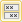
\includegraphics[width=.05\textwidth]{felder-mit-inhalt-symbol}
	\vspace{-35pt}
\end{wrapfigure}

\noindent
Felder der Inhalt blendet \textbf{alle} Felder, die mit einem Wert belegt sind, ein. Dies kann hilfreich sein um einen daran zu erinnern welche Felder mit Werten zu belegen sind. Es kann einen auch einen etwas tieferen Verständnis der Abläufe in Untis geben, denn es werden nicht nur Benutzer gefüllte Werte angezeigt sondern auch die Werte, die dynamisch vom Programm berechnet sind.\\

\subsubsection{Fenster Aktualisieren}
{\small\textit{verfügbar in Stammdaten und Unterricht Ansichten\\}\par}

\begin{wrapfigure}{r}{.05\textwidth}
	\vspace{-50pt}
	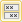
\includegraphics[width=.05\textwidth]{felder-mit-inhalt-symbol}
	\vspace{-35pt}
\end{wrapfigure}

\noindent
Aktualisiert das Fenster. Untis sucht nach lokale und externe Änderungen und pflegt gefundene Datensätze sortiert ein. \\

\subsubsection{Klassenzeitraster}
{\small\textit{verfügbar in Gruppen-Stammdaten Ansichten\\}\par}

\begin{wrapfigure}{r}{.05\textwidth}
	\vspace{-50pt}
	
\includegraphics[width=.05\textwidth]{klassenzeitraster-symbol}
	\vspace{-35pt}
\end{wrapfigure}

\noindent
Hier wird ein Fenster geöffnet in dem man den Tagesablauf einer Gruppe anhand der assoziierte Raster für die automatische/optimierte Planung festlegen können sollte. Diese scheint nicht vollständig implementiert zu sein. Bitte nicht benutzen.\\

\subsubsection{Koppeln}
{\small\textit{verfügbar in Unterricht Ansichten\\}\par}

\begin{wrapfigure}{r}{.05\textwidth}
	\vspace{-50pt}
	
\includegraphics[width=.05\textwidth]{koppeln-symbol}
	\vspace{-35pt}
\end{wrapfigure}

\noindent
Dieser Symbol öffnet einen Ansicht, in dem mehrere getrennte Unterrichte zu einem Unterricht mit mehrere Kopplungszeilen zusammenfügen kann. Nähere Informationen dazu in Sektion !!!!!!!.\\

\subsubsection{Lehrer-Vorschlag}
{\small\textit{verfügbar in Unterricht Ansichten\\}\par}

\begin{wrapfigure}{r}{.06\textwidth}
	\vspace{-50pt}
	
\includegraphics[width=.06\textwidth]{lehrer-vorschlag-symbol}
	\vspace{-35pt}
\end{wrapfigure}

\noindent
Der Lehrer-Vorschlag bietet Ihnen einen kleinen Menü an in dem die Möglichkeiten des Lehrer-Vorschlag-Ansichts, das Dozent-Feld zu leeren und der Vorjahres-Lehrer zu verwenden stehen.\\
\\
Der Lehrer-Vorschlag Ansicht listet alle Dozenten anhand ihre von Untis eingetragene/kalkulierte Ist, Soll und Ist-Soll Werte. Diese kann von nutzen sein wenn man nach einem Dozent mit freien Kapazitäten sucht. Standardmäßig werden die Dozenten nach Ihre noch zu fühlende Stunden aufgelistet, jedoch können diese Angaben nach allen Spalten sortiert werden.\\
\\
Die Option Vorjahres-Lehrer bezieht sich auf Klassen-Lehrer wie man von der Grundschule oder Gymnasium kennt und ist für unsere Zwecke nicht zu gebrauchen.\\

\subsubsection{Normalform Anzeigen}
{\small\textit{verfügbar in allen Fenster Ansichten\\}\par}

\begin{wrapfigure}{r}{.05\textwidth}
	\vspace{-50pt}
	
\includegraphics[width=.05\textwidth]{normal-form-anzeigen-symbol}
	\vspace{-35pt}
\end{wrapfigure}

\noindent
Die Schaltfläche Normalform Anzeigen bewirkt, dass die Breite des Fensters passt sich die Höhe und Breite der angezeigten Zeilen und Spalten. Bei eine geringe Anzahl an Einträge wird die Höhe des Fensters ggf. schrumpfen. Wohingegen bei vielen Zeilen könnte die komplette Höhe der Arbeitsfläche eingenommen werden.\\
\\
Zusätzlich bei manche Ansichten führt das Klicken auf diesem Symbol eine Art Zurücksetzen durch. Bei Gruppenstundenpläne zum Beispiel wird man zurück zum Gruppenplan vom letzten angeklickten Unterricht. Diese kann eine ganz andere Gruppe sein als die mit der man angefangen hat.\\

\subsubsection{Raum Zuordnen / Löschen}
{\small\textit{verfügbar in Unterricht Ansichten\\}\par}

\begin{wrapfigure}{r}{.05\textwidth}
	\vspace{-50pt}
	
\includegraphics[width=.05\textwidth]{raum-zuordnen-loschen-symbol}
	\vspace{-35pt}
\end{wrapfigure}

\noindent
Dieses Symbol, oder der entsprechende Unterrichtsstunde Kontextmenüeintrag, öffnet die Ansicht ``Raum zuordnen / löschen" für die im Stundenplan selektierte Stunde. Hier kann man alle Räume einer Periode anschauen mit ausgewählte Informationen wie ``Besetzt" (ob der Raum schon in der Stunde verplant ist), Kapazität (Anzahl der Sitzplätze), ob ein Raum als Ausweichraum für den gewünschten Raum eingetragen ist, soweie die Raumgruppenzugehörigkeit, falls eingetragen.\\

\begin{wrapfigure}{r}{0.3\textwidth}
	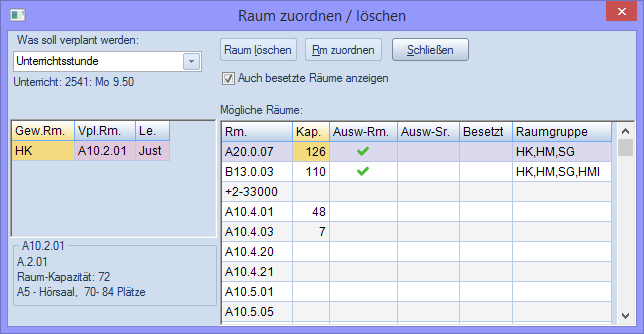
\includegraphics[width=.29\textwidth,right]{raum-zuordnen-loschen}
	\vspace{-15pt}
	\caption{Raum zuordnen / löschen}
	\label{fig:raum-zuordnen-loschen}
\end{wrapfigure}

\noindent
Man kann Raume zuordnen in dem man ein Raum selektiert und den Knopf Raum 

\subsubsection{Schuljahreskalendar}
{\small\textit{verfügbar in Stammdaten (ausser Fächer) und Unterricht Ansichten\\}\par}

\begin{wrapfigure}{r}{.05\textwidth}
	\vspace{-50pt}
	
\includegraphics[width=.05\textwidth]{schuljahreskalendar-symbol}
	\vspace{-35pt}
\end{wrapfigure}

\noindent
Bei Stammdaten öffnet dieser Symbol die Absenzen Ansicht wo man die nicht verfügbaren Tage einer Ressource eintragen kann. Leider scheint diese Funktion nicht vollständig implementiert zu sein und ist an mehreren Stellen fehlerhaft, bitte nicht benutzen.\\
\\
Bei Unterrichte wird tatsächlich den Schuljahreskalender geöffnet. Hier wird einen die Ablauf des Unterrichts angezeigt abhängig vom Unterrichtsgruppe, Von- und Bis- Datum. Der Verlauf lässt sich aber nicht von dieser Ansicht beeinflussen lassen.\\

\subsubsection{Seitenlayout}
{\small\textit{verfügbar in Stammdaten und Unterricht Ansichten\\}\par}

\begin{wrapfigure}{r}{.06\textwidth}
	\vspace{-50pt}
	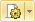
\includegraphics[width=.06\textwidth]{seitenlayout-symbol}
	\vspace{-35pt}
\end{wrapfigure}

\noindent
Ein klick auf dieses Symbol eröffnet ein kleines Menü in dem Seitenanischt und Seitenlayout stehen. Seitenansicht ist die drückbare Ausgabe der in dem Fenster erhaltene Informationen, wohingegen Seitenlayout beinhaltet die Gestaltungseinstellungen dessen. Mehr Informationen dazu finden Sie im Sektion !!!!!!.\\

\subsubsection{Sortieren (automatische)}
{\small\textit{verfügbar in Stammdaten und Unterricht Ansichten\\}\par}

\begin{wrapfigure}{r}{.05\textwidth}
	\vspace{-50pt}
	
\includegraphics[width=.05\textwidth]{sortieren-symbol}
	\vspace{-35pt}
\end{wrapfigure}

\noindent
Das Sortieren-Symbol öffnet eine weitere Ansicht, die das Automatische sortieren ermöglicht. Hier kann man mehrere Spalten auswählen die als Sortierkriterien dienen können, sowie die Sortierrichtung dieser.\\

\begin{wrapfigure}{r}{0.3\textwidth}
	\vspace{-24pt}
	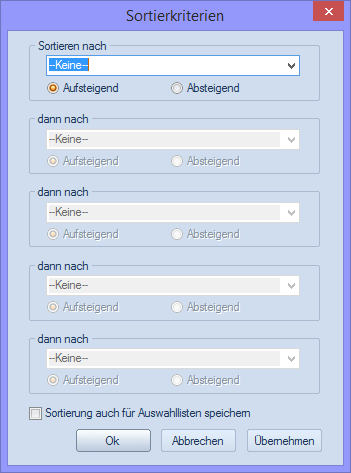
\includegraphics[width=.29\textwidth,right]{sortierkriterien}
	\vspace{-15pt}
	\caption{Sortierkriterien}
	\label{fig:sortierkriterien}
\end{wrapfigure}

\noindent
Das eingestellte Sortierverhalten kann mit ``Ok" oder ``Übernahme" bestätigt werden. Obwohl das Verhalten \textit{permanent} gespeichert wird, kann es nicht nach dem Schließen des Fensters nicht nochmal eingesehen werden. Sollte die Sortierkriterien Ansicht neu aufgerufen werden nach dem Schließen werden keine der bereits gespeicherte Einstellungen angezeigt und, sollte man sie nicht neu einstellen, gehen sie nach dem Schließen der Ansicht egal wie verloren.\\
\\
Ansichten, die mit Stammdaten assoziiert sind, kann man auch ein Häkchen unten setzen. Diese bewirkt, dass die gespeicherte Sortierung auch für Auswahlboxen für die Ressourcentyp eingehalten wird. Jedoch egal in welcher Zustand das Sortieren sich befindet müssen neue solche Elemente manuell-automatisch, sprich die Sortierung neu einpflegen mit Häkchen, damit die gewünschte Sortierung neue Elemente berücksichtigt in Auswahlboxen.\\

\subsubsection{Stundenplanvergleich}
{\small\textit{verfügbar in Stundenplan Ansichten\\}\par}

\begin{wrapfigure}{r}{.05\textwidth}
	\vspace{-50pt}
	
\includegraphics[width=.05\textwidth]{stundenplan-vergleich-symbol}
	\vspace{-35pt}
\end{wrapfigure}

\noindent
_\begin{Dieser Symbol soll es ermöglichen zwei Stundenpläne zu vergleichen. Laut dem Tooltip soll

\subsubsection{Unterrichtsstunde Fixieren}
{\small\textit{verfügbar in Stundenplan Ansichten\\}\par}

\begin{wrapfigure}{r}{.05\textwidth}
	\vspace{-50pt}
	
\includegraphics[width=.05\textwidth]{unterrichtsstunde-fixieren-symbol}
	\vspace{-35pt}
\end{wrapfigure}

\noindent
Sollte man die automatische/optimierte Planung benutzen, verhindert das Betätigen dieses Symbols, dass der geplante Unterricht von diese Planungsvorgänge geändert wird.\\

\subsubsection{Unterrichtsvergleich}
{\small\textit{verfügbar in Unterricht Ansichten\\}\par}

\begin{wrapfigure}{r}{.05\textwidth}
	\vspace{-50pt}
	
\includegraphics[width=.05\textwidth]{unterrichtsvergleich-symbol}
	\vspace{-35pt}
\end{wrapfigure}

\noindent
Dieser Symbol lässen sich Unterrichte mit dem selben ID unterschiedliche Perioden vergleichen. Einmal gedrückt öffnet sich ein Ansicht in dem man die Periode auswählen kann, sowie wie die Ergebnisse dargestellt werden. Da wir mit viel Fluktuation in der Zahl der Studenten, angebotenen Fächer, Studentengruppen und eingesetzte Dozierende bringt dieser Funktion uns nicht viel.\\

\subsubsection{Zeitwünsche}
{\small\textit{verfügbar in Stammdaten und Unterricht Ansichten\\}\par}

\begin{wrapfigure}{r}{.05\textwidth}
	\vspace{-50pt}
	
\includegraphics[width=.05\textwidth]{zeitwunsche-symbol}
	\vspace{-35pt}
\end{wrapfigure}

\noindent
Zeitwünsche öffnet eine weitere Fenster in dem man Präferenzen zu der Zeiten, in den Stammdaten zur Verfügung stehen oder Unterrichte gehalten werden gehalten werden sollen, angeben kann. Diese Präferenzen sind abgebildet auf numerische Werte zwischen -3 und +3 mit einem großen 'X' anstelle der 0 Wert. Im wesentlichen dienen diese Angaben die automatische/optimierte Stundenplanerstellung. Doch die Angabe -3 hat eine besondere Stellenwert, in der er als absolute Sperre gilt. Einst belegt mit diesem Wert, wird Untis einen Fehler, sobald man manuell versucht einen Unterricht zu einer gesperrten Zeit zu planen, melden.\\

\begin{wrapfigure}{r}{0.3\textwidth}
	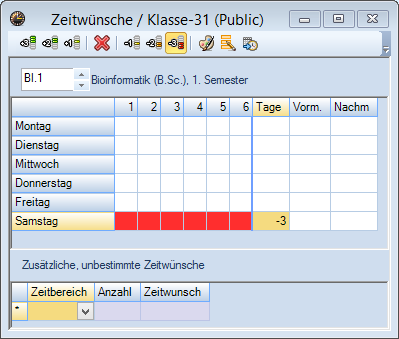
\includegraphics[width=.29\textwidth,right]{zeitwunsche-gruppen}
	\vspace{-15pt}
	\caption{Zeitwünsche Gruppen}
	\label{fig:zeitwunsche-gruppen}
\end{wrapfigure}

\noindent
Die Zeitwünsche Ansichten haben ein paar wesentlichen Binnendifferenzen im Abhängigkeit von aufrufende Ansicht, ggf. Ressourcentyp dessen und die Verwendung der sogenannte Multi-Zeitraster. Im Figure \ref{fig:zeitwunsche-gruppen} sehen wir den Zeitwünsche Ansicht für die Ressource Gruppen. Im Hauptteil des Fensters steht mittig der Zeitraster des Elements. Hier kann man die Werte Blockweise Eintragen in dem Unterrichte für diese Ressource stattfinden, bzw. nicht-stattfinden sollen. Bei Gruppen und Dozenten Zeitwünsche hat man eine erweiterte Hilfsmittel in dem man für ganze Zeitbereiche, Ganztags, Vormittags oder Nachmittags, diese Werte setzen kann. Räume und Fächer Zeitwünsche haben kein solches Hilfsmittel.\\
\\
Da Gruppen immer mit einem festen Zeitraster gebunden sind wird immer diese in dem entsprechenden Zeitwünsche Ansicht angezeigt. Bei Dozenten, Räume und Fächer hingegen kann kein eindeutiger Zeitraster angegeben werden. Sollte mehrere Raster vorliegen, sehen ihre Zeitwünsche komplizierter aus, wie in Figure \ref{fig:zeitwunsche-multiraster} veranschaulicht. Hier muss man entsprechende Zeitbereiche mit den jeweiligen Wert belegen. Die aktuelle Position des Cursors (in Minuten) wird in der erste Reihe/Spalte angezeigt.

\begin{figure}[h]
	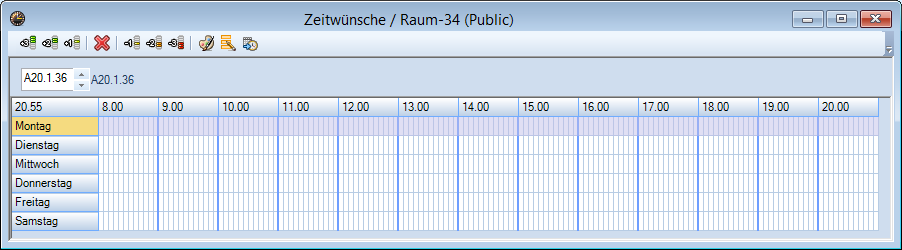
\includegraphics[width=1\textwidth]{zeitwunsche-multiraster}
	\vspace{-15pt}
	\caption{Zeitwünsche Multi-Zeitraster}
	\label{fig:zeitwunsche-multiraster}
\end{figure}

\begin{wrapfigure}{r}{0.3\textwidth}
	\vspace{-14pt}
	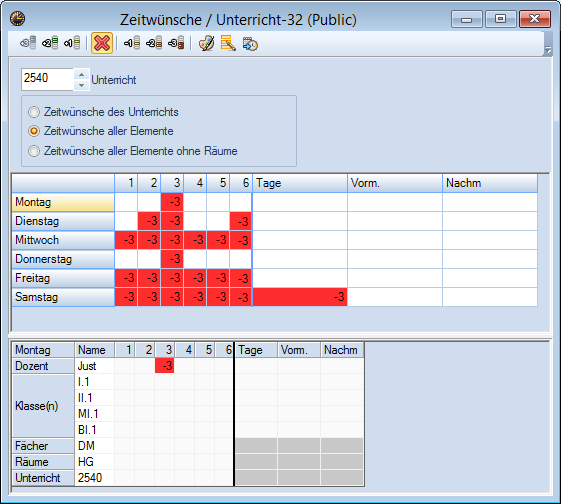
\includegraphics[width=.29\textwidth,right]{zeitwunsche-unterricht}
	\vspace{-15pt}
	\caption{Zeitwünsche Unterrichte}
	\label{fig:zeitwunsche-unterricht}
\end{wrapfigure}

\noindent
Unterrichte sind über die zugewiesenen Klassen auch an einem festen Raster gebunden und wie Gruppen und Dozenten kann man auch ganze Zeitbereiche mit einem Wert belegen. Man hat hier die Wahl zwischen drei Verschiedene Darstellungsmöglichkeiten: Unterricht, alle Elemente und alle Elemente ohne Räume. Bei allen drei Möglichkeiten werden automatisch die Zeitwunsch-Werte der assoziierte Ressourcen tageweise unten dargestellt. In Figure \ref{fig:zeitwunsche-unterricht} z.B. sieht man in der Liste der Ressourcen unten eine Sperre bei Frau Just Montags im 3. Block. Bei alle Elemente und ohne Räume werden die Zeitwünsche der assoziierte Ressourcen direkt als die des Unterrichts angezeigt. 

\subsection{Fenster-Aktionen}

\subsubsection{Filter}

\subsubsection{Sortieren}

\subsubsection{Neu}

\subsubsection{Serienänderungen}